\documentclass{article} % This line defines the type of document. 'article' is a common class for small documents.
\usepackage[margin=1.15in]{geometry}
\usepackage{graphicx}
\usepackage{titlesec}
\usepackage{caption}
% \usepackage{hyperref}
\usepackage[colorlinks=true, linkcolor=blue, citecolor=blue, urlcolor=blue]{hyperref}
\usepackage{amsmath}

% \emergencystretch=3em

% Set paragraph indentation to zero
\setlength{\parindent}{0pt}

\titleformat{\section}
  {\normalfont\large\bfseries}{\thesection}{1em}{}

\begin{document} % This line marks the beginning of the document content.


\noindent\makebox[\linewidth]{\rule{\textwidth}{1pt}} 
\vspace*{0mm} % adds vertical space before the title
\begin{center}
    \Large\textbf{Toy Models of Superposition Replication and Findings}
\end{center}
\vspace*{2mm} % adds vertical space before the title
\noindent\makebox[\linewidth]{\rule{\textwidth}{1pt}}
\vspace*{0mm}

% \noindent
\noindent\textbf{Zephaniah Roe} \hfill \texttt{zroe@uchicago.edu}\\
\noindent\text{Undergraduate Student at the University of Chicago} \\


% \hfill
% \begin{minipage}[b]{0.4\linewidth}
%     \raggedleft
%     \texttt{G.RAS@DONDERS.RU.NL}
% \end{minipage}

% \vspace{2cm} % adds some vertical space before the main content


\begin{abstract}
\begin{quote}
    \textit{Toy Models of Superposition}\cite{elhage2022toy} is a groundbreaking 
    paper published by researchers affiliated with Anthropic and Harvard University in 2022. By 
    investigating small models with under 100 neurons, the paper demonstrates 
    that neural networks can represent more features than they have dimensions. 
    Additionally, they use these so-called ``toy models'' to understand the 
    relationship between how neural networks are trained and how they represent 
    the data internally. Because the paper is quite extensive, this
    replication only focuses on reproducing the most important results from the  
    introduction and sections 2 and 3 of the original paper. It also includes 
    some commentary on section 1.
\end{quote}
\end{abstract}
\section{Introduction}
\textit{Toy Models of Superposition} motivates the idea of superposition with the following graphic:

\begin{figure}[h]
    \centering
    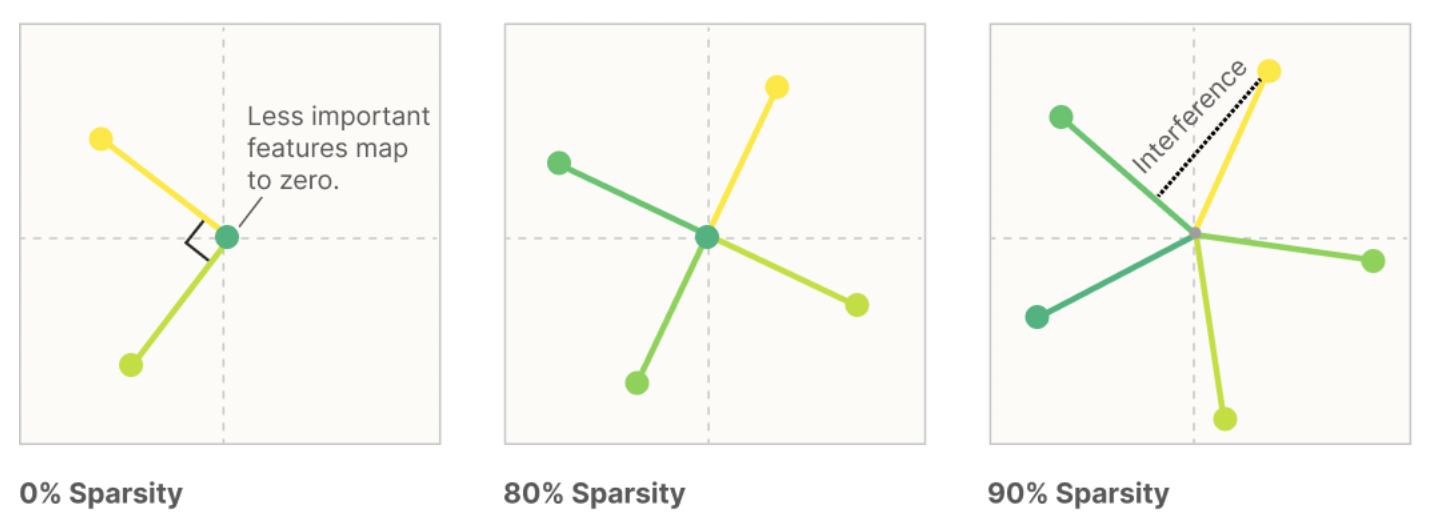
\includegraphics[width=0.55\linewidth]{introduction/images/introduction_anthropic_graphic_.png}
    \captionsetup{font=footnotesize} % Set the font size for this caption
    \caption{
        Graphic from \textit{Toy Models of Superposition} showing superposition
        in 2D.
    }
    \label{fig:section1_anthropic}
\end{figure}

The basic idea is this: if you think of each feature as being represented inside of a
neural network by a direction, you can graph these directions and observe them.
By doing this, the authors of \textit{Toy Models of Superposition} demonstrate that
the internal structure of a model depends on the sparsity of its training data.
A replication of this phenomenon can be found below and the code used to 
generate it can be found 
\href{https://github.com/zroe1/toy_models_of_superposition/blob/main/section_1/section_1.ipynb}{here}.\\ 

\begin{figure}[h]
    \centering
    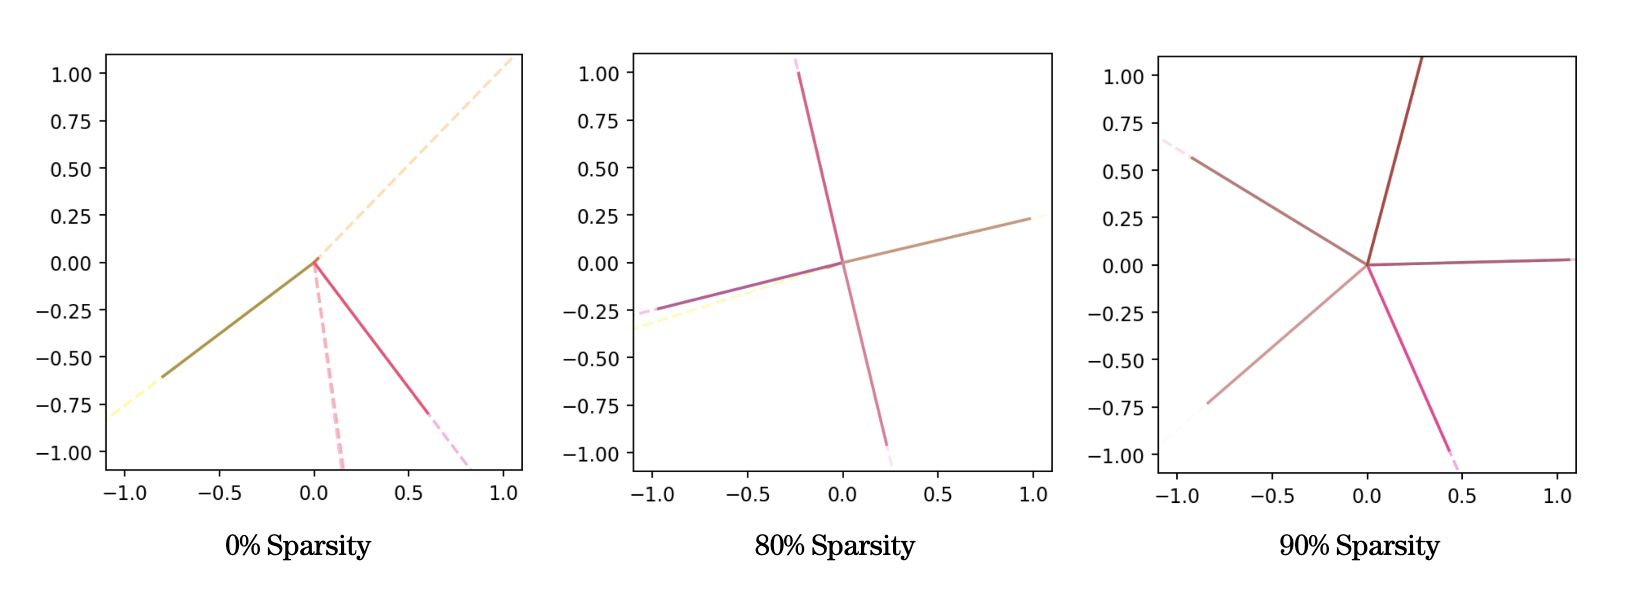
\includegraphics[width=0.6\linewidth]{introduction/images/introduction_replicated_graphic.png}
    \captionsetup{font=footnotesize} % Set the font size for this caption
    \caption{Replication of Figure~\ref{fig:section1_anthropic}}
    \label{fig:section1_replication}
\end{figure}

The model studied in  Figure~\ref{fig:section1_replication} is designed such that 
each column in the weight matrix corresponds to a  given input. The weight
matrix in this example contains only 2 neurons, so each column can be graphed as
a 2D vector. Observing these vectors while increasing the sparsity of the model's input reveals
that the model can represent five features despite having only 2 neurons. This 
kind of representation is what the authors call "superposition." In future sections we will study 
superposition extensively and reproduce this phenomenon in larger networks.

\section{Background and Motivation}

Before studying superposition in detail, the authors of  \textit{Toy Models of Superposition}, 
provide context by explaining concepts and defining terms. In this section, I 
provide some additional commentary on the definitions and explanations the authors use. \\

\textbf{(1) Defining Features: }\textit{Toy Models of Superposition}
defines features broadly as ``properties of the input which a sufficiently large 
neural network will reliably dedicate a neuron to representing.'' The authors do
however describe this definition as ``slightly circular'' and note that they are
not ``overly attached to it.'' I find the definition especially problematic because 
certain architectures may be incentivized to ignore an aspect of the input that 
differently designed models may "want" to internally represent. It is unclear to me whether
there is sufficient evidence to support the idea of a sort of ground truth for 
features. As a result, I propose an alternative definition: features are aspects 
of the input that a neural network represents accurately with a significantly higher probability than 
a randomly initialized network. In other words, features are parts of the input 
that a model determines to be important enough to represent internally.\\

\textbf{(2) Role of Linear Representations in Neural Networks: }The original authors
of the paper study interpretability by trying to understand the linear representations
within neural networks. It is worth noting that this isn't the only way to approach
mechanistic interpretability research. Understanding the role of non-linearities 
at each level is likely also very important (and perhaps more neglected).\newline\newline
\textbf{(3) Defining Superposition: } The original paper has a compelling yet
simple definition for Superposition: ``Roughly, the idea of 
superposition is that neural networks `want to represent more features than they 
have neurons', so they exploit a property of high-dimensional spaces to 
simulate a model with many more neurons.'' This is the definition I will use
throughout this paper.

\section{Demonstrating Superposition}

In the introduction, the authors of the original paper proved that models with 
two neurons could exhibit superposition (this result was reproduced in Figure~\ref{fig:section1_replication}).
Later in the paper, however, the authors demonstrate that superposition
is also observed in models with more than two neurons. Specifically they begin 
by exploring two models with a weight matrix $W_{5 \times 20}$: a linear model defined by 
$W^TWx + b$ and a ReLU model defined by ReLU($W^TWx + b$). The objective of both
models was to reconstruct the input $x$. The authors used a weighted mean squared
error loss function making accurately representing some features more important
than others. For more information about the loss see section 2 of the original
paper.\\

While the model without an activation function appears to only represent features
orthogonally, the authors claim that the ReLU model can exhibit superposition
if it is trained on sparse enough data. Because we defined each weight matrix with 5 neurons ($W_{5 \times 20}$)
this claim cannot be validated by graphing features in 2D like in Figure~\ref{fig:section1_replication}. 
But by graphing $W^TW$, superposition in the ReLU model can be shown visually in Figure~\ref{fig:section3_anthropic}. 
In this figure, positive numbers in the matrix $W^TW$ are labeled red while 
negative ones are colored blue. They also graph the length of each feature by treating 
each column in $W$ as a vector. Features that are orthogonal to others in $W$ are 
labeled black while features that aren't are labeled yellow
(the exact details for how this is calculated is discussed in \ref{sec:calc_super}).\\

\begin{figure}[h]
    \centering
    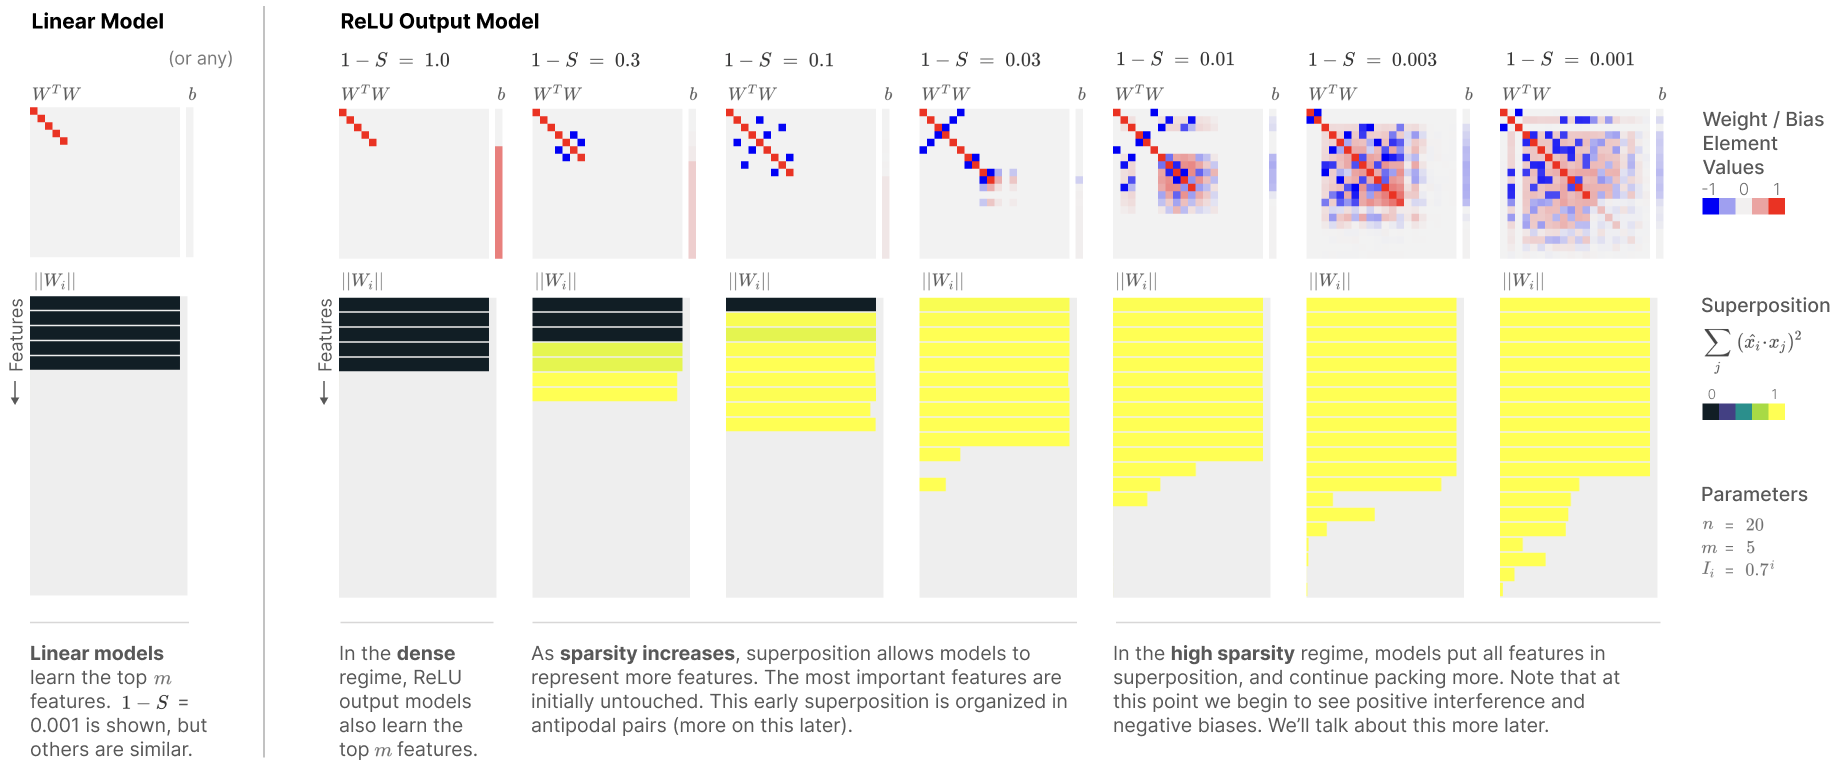
\includegraphics[width=0.9\linewidth]{demonstrating_superposition/images/anthropic_section3.png}
    \captionsetup{font=footnotesize} % Set the font size for this caption
    \caption{Superposition in linear and ReLU models from \textit{Toy Models of Superposition}\cite{elhage2022toy}}
    \label{fig:section3_anthropic}
\end{figure}

The visualization of $W^{T}W$ (top of Figure~\ref{fig:section3_anthropic}) and the 
chart of feature representations (bottom of the figure) both show that by increasing sparsity, the 
ReLU model ceases to represent features orthogonally. The yellow bars shown in the models
on the right side of the figure illustrate that the model maps all its features 
in superposition. This is also shown in the graphs of the weight matrices $W^{T}W$ for
sparse models in Figure~\ref{fig:section3_anthropic}. These 
representations appear to show the model embedding more than 5 features, but 
the representation is noisy.\\ 

The first step in replicating these findings was to train the linear and ReLU
models that don't perform computation in superposition. The
objective of each model was to reconstruct the input $x$. Both 
models were trained with the Adam optimizer (learning rate = $1*10^{-3}$) on 
20,000 batches of 256 examples.

\begin{figure}[h]
    \centering
    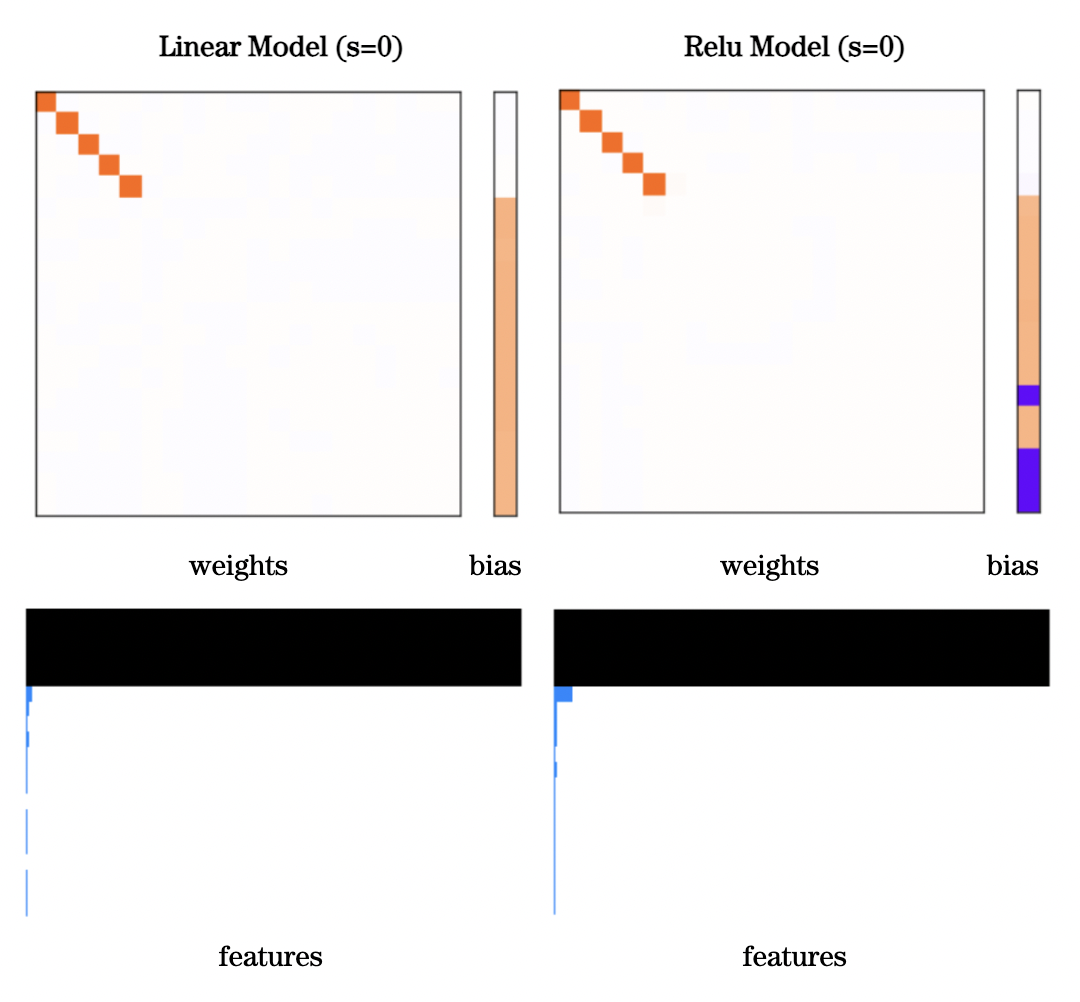
\includegraphics[width=0.4\linewidth]{demonstrating_superposition/images/relu_linear_0_sparsity.png}
    \captionsetup{font=footnotesize, width=0.7\linewidth} % Set the font size for this caption
    \caption{The generated graphics show that the linear and ReLU models trained on
    dense inputs represent only five features (one for each dimension in the model).}
    \label{fig:relu_linear_0}
\end{figure}

Note that in Figure~\ref{fig:relu_linear_0}, I use orange to indicate
positive numbers and purple to indicate negative ones. This is different from
the red and blue in Figure~\ref{fig:section3_anthropic} to distinguish my work 
from that of the original authors. Similarly, while the original authors use 
yellow to indicate features in superposition, I use blue (This is hard to see in 
Figure~\ref{fig:relu_linear_0} but it will be more obvious going forward).

\subsection{Calculating Superposition}
\label{sec:calc_super}

The models in Figure~\ref{fig:relu_linear_0} do not exhibit superposition. They
encode the five most important features orthogonally (one feature for each
neuron in the model). In this section, we will be investigating models
that do not behave in this way, instead encoding features as vectors that interfere
with each other. The model explored in this section is defined by the same architecture
and objective as the models in Figure~\ref{fig:relu_linear_0}. The difference
is that the models in this section are trained on sparse input data and, as a
result, map features internally in superposition. \\

In order to explain this phenomenon and demonstrate how models with sparse input
are able to represent features in superposition, it will be useful to dive into 
the math behind the concept of feature interference. The extent to which 
features interfere with each other is defined by the following equation:

\begin{equation}
\label{eq:my_equation}
\text{Interference} = \sum_{j \neq i} (\hat{W}_i \cdot \hat{W}_j)^2
\end{equation}

For a given column $i$ in weight matrix $W$, interference is calculated by taking
the dot product with every other column in $W$. Non-zero dot products indicate
that the columns in $W$ are not orthogonal. As a result, summing these dot 
products gives a general idea of how much the network is representing a given
feature in superposition. Note that $\hat{W}_i$ is the unit vector for $W_i$. 
This is necessary because when calculating interference, we are interested in
the direction of a given feature, not its length.\newline

In Figure~\ref{fig:sparsity_1}, the length of a feature (calculated by taking the
length of the vector $W_i$) determines the width of the bars in the feature
graph (shown in the bottom half of the figure). The interference equation (Equation~\ref{eq:my_equation}) determines the
color of the columns: black indicates a low value for interference
while blue indicates a higher value. This means that blue bars show that a given feature is represented
in superposition while black bars indicate that the feature is mapped orthogonally.
    

\begin{figure}[h]
    \centering
    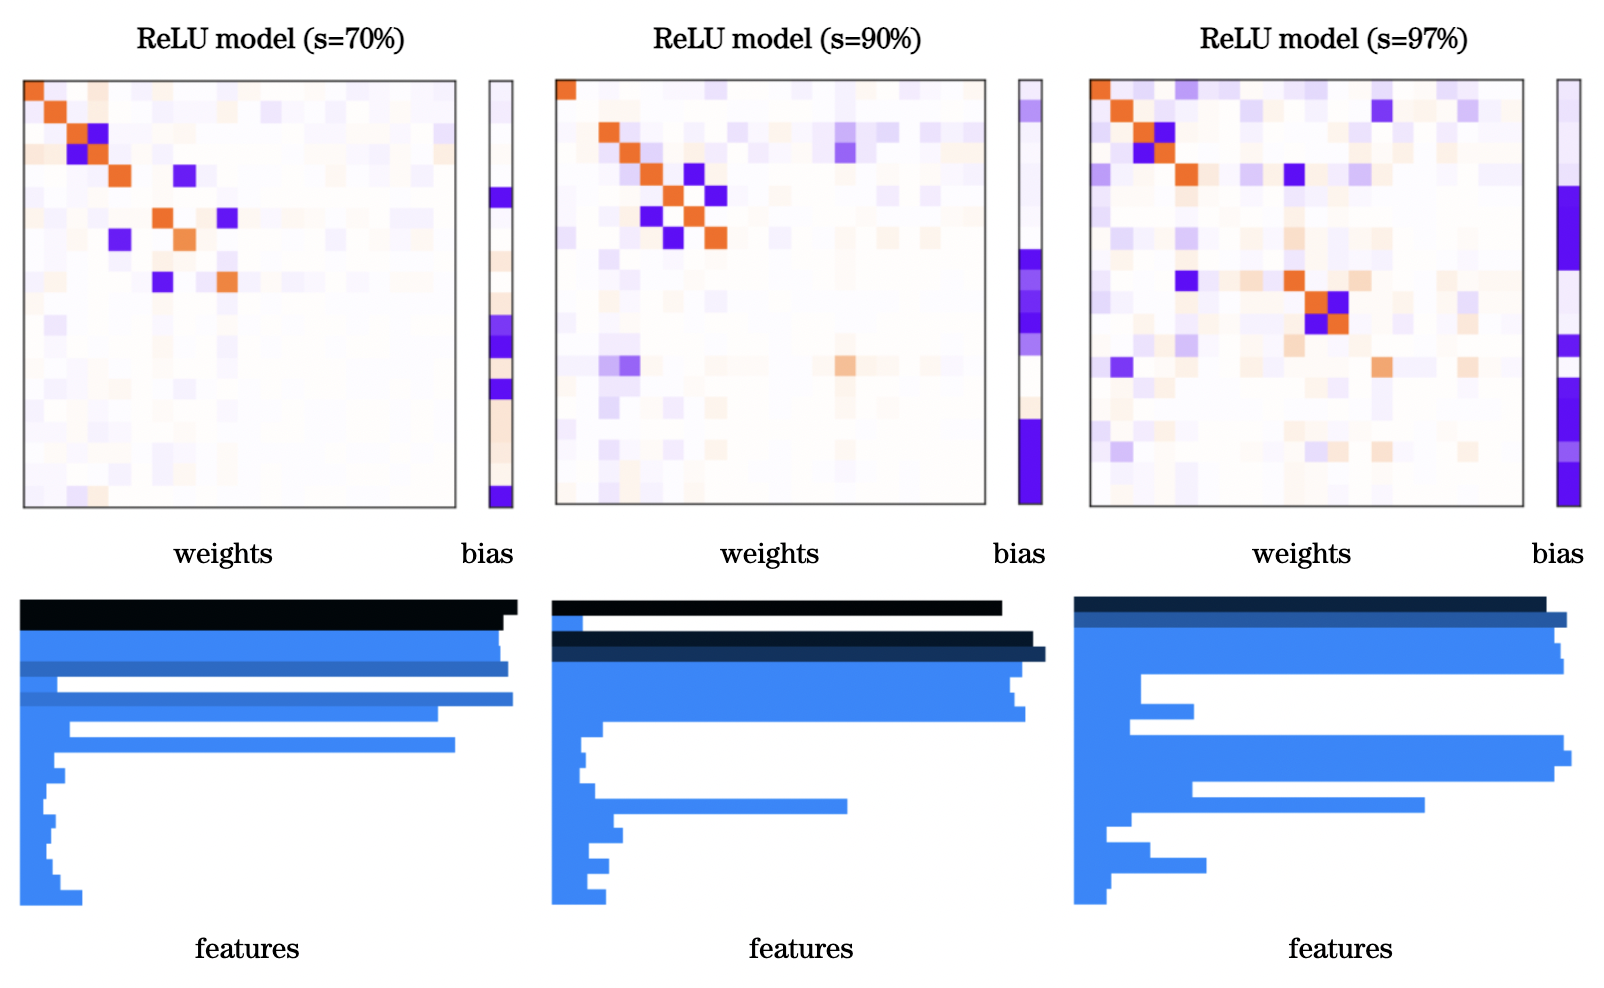
\includegraphics[width=0.75\linewidth]{demonstrating_superposition/images/sparsity_superposition1.png}
    \captionsetup{font=footnotesize, width=0.71\linewidth} % Set the font size for this caption
    \caption{
        Superposition is observed in models trained on 70\%, 90\% and 97\% 
        sparse inputs (code to generate these figures can be found 
        \href{https://github.com/zroe1/toy_models_of_superposition/blob/main/section_1/section_1.ipynb}{here}). 
        The 70\% and 90\% sparse models were trained on 50,000 batches of 256 
        examples with the ``RMSProp'' optimizer (learning rate = $10^{-2}$). The 
        97\% sparsity model was trained on 100,000 batches of 256 examples using 
        the Adam optimizer (learning rate = $10^{-2}$).
    }
    \label{fig:sparsity_1}
\end{figure}

Unlike the models with 0\% sparsity in Figure~\ref{fig:relu_linear_0}, the models
in Figure~\ref{fig:sparsity_1} have higher levels of sparsity and, as
a result, leverage superposition. The bottom half of Figure~\ref{fig:sparsity_1}
shows that these models represent far more features than the models in
Figure~\ref{fig:relu_linear_0}, but by doing so, they are forced to represent many 
of their features in superposition. The models only have 5 neurons so if they 
``want'' to represent more than 5 features, they can't represent each feature 
orthogonally. This tradeoff is intuitively more attractive when the model is
trained on sparse inputs because it is less likely that the model will be fed
a combination of inputs that cause feature representations to conflict (because
a significant percentage of the input is 0).


\subsection{Models Trained on Very Sparse Data}

As sparsity is increased to almost 100\% the models stop representing any features
orthogonally. This is displayed in Figure~\ref{fig:sparsity_2} where models are
trained on 99\%, 99.7\% and 99.9\% sparse inputs.

\begin{figure}[h]
    \centering
    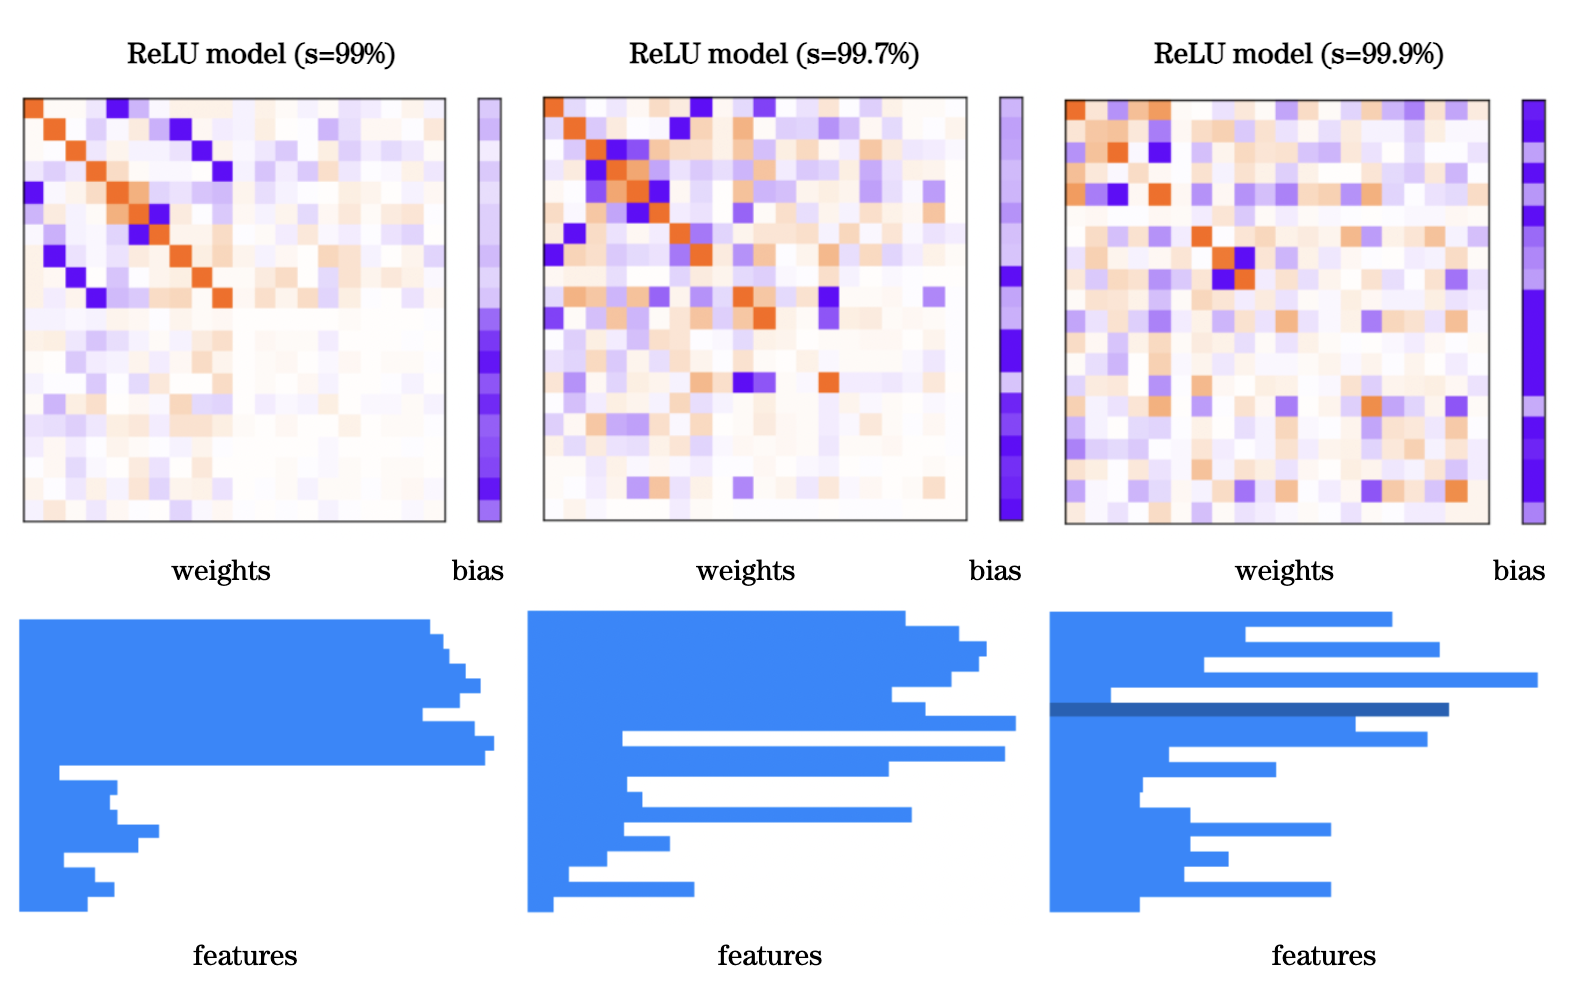
\includegraphics[width=0.75\linewidth]{demonstrating_superposition/images/sparsity_superposition2.png}
    \captionsetup{font=footnotesize, width=0.7\linewidth} % Set the font size for this caption
    \caption{
        When models are trained on sufficiently sparse data, all feature
        representations are in superposition. The models in the figure were
        trained on 100,000 batches of 256 examples using the Adam optimizer 
        (learning rate = $10^{-2}$).
    }
    \label{fig:sparsity_2}
\end{figure}

The representations of $W^{T}W$ of these very sparse models (shown in the top
half of Figure~\ref{fig:sparsity_2}) is far less clean than previous
representations we have seen. This is the same trend the original authors
found when increasing sparsity of these models (Figure~\ref{fig:section3_anthropic}
illustrates how the original authors displayed this visually). \\

The feature representations, shown in the bottom half of Figure~\ref{fig:sparsity_2},
are also consistent with the findings of \textit{Toy Models of Superposition}.
Like the investigation from the original paper, these feature representations 
show no features mapped orthogonally (recall that features that interfere with
each other are shown in blue). \\

\subsection{Scaling Results to Larger Models}

In the previous subsections, we have explored superposition in models with 5
neurons and 20 inputs. This proves that the phenomenon we observed in Figure~\ref{fig:sparsity_2}
applies to models with more than 2 neurons. The original paper expanded this 
finding by also studying models with 20 neurons and 80 inputs (Figure~\ref{fig:section3_anthropic2}). \\

\begin{figure}[h]
    \centering
    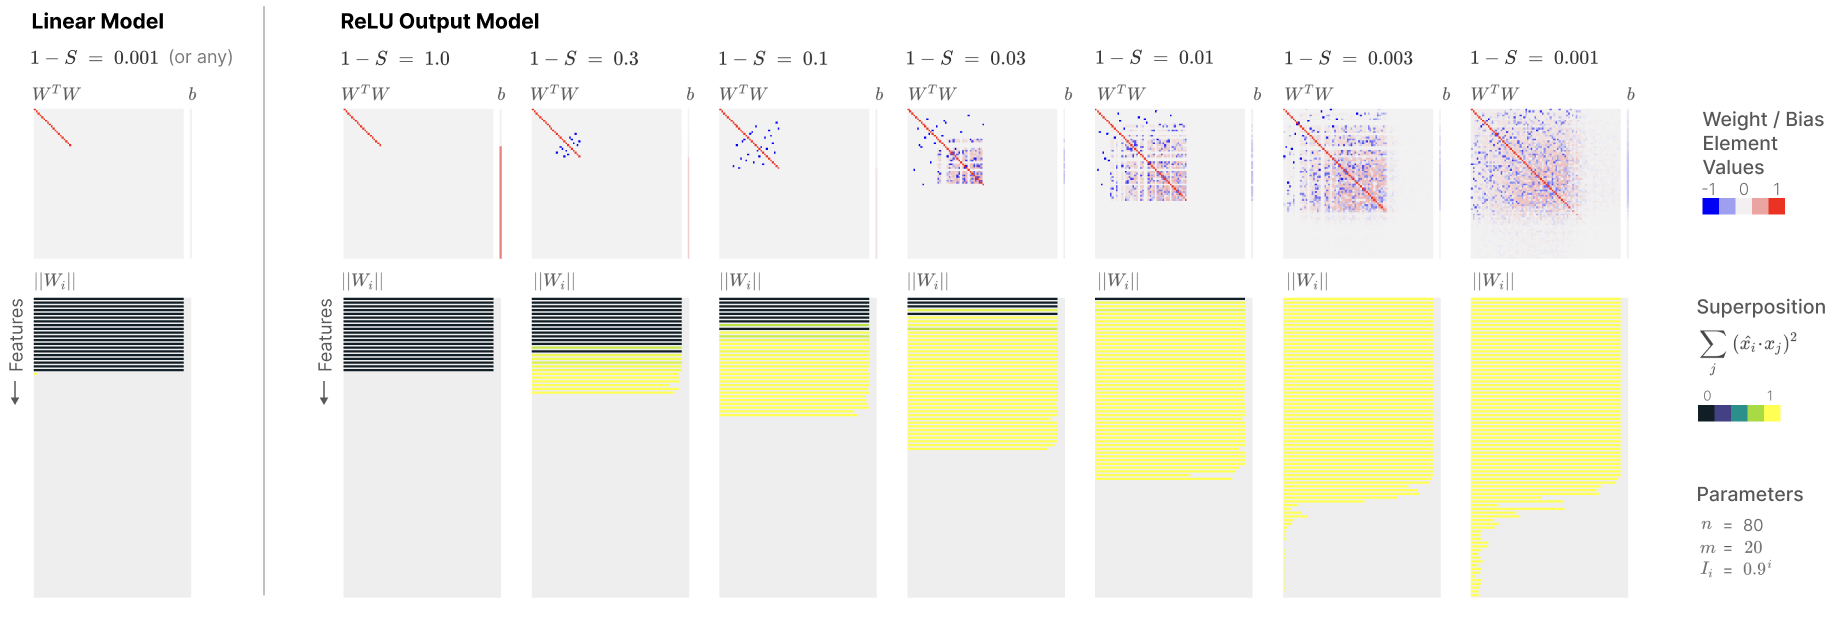
\includegraphics[width=0.99\linewidth]{demonstrating_superposition/images/anthropic_section3_part2.png}
    \captionsetup{font=footnotesize, width=0.7\linewidth} % Set the font size for this caption
    \caption{
        Superposition in models with 20 neurons and 80 inputs from \textit{Toy Models of Superposition}\cite{elhage2022toy}
    }
    \label{fig:section3_anthropic2}
\end{figure}

The original authors report that this experiment produced ``qualitatively similar''
results compared to the models with 5 neurons and 20 inputs. Because this experiment 
is almost identical to the previous ones, and because I would not expect to find 
results that conflict with the original paper, I have excluded this experiment 
from this replication. \\

\section{Superposition as a Phase Change}

The author's of \textit{Toy Models of Superposition} claim that superposition
can be thought of as a kind of ``phase change.'' Figure~\ref{fig:section4_anthropic}
shows a phase diagram for single-neuron models with 2 inputs. The models studied were
defined by ReLU($W^TWx + b$) and trained to simply reconstruct their inputs. The authors 
used a weighted mean squared error loss where the importance of 
the second output was varied between 0.1 and 10. The relative importance of this
second output represents the x-axis for the graphs in Figure~\ref{fig:section4_anthropic}.
The y-axis reflects the model's feature density---in other words, the probability
that a given input will be non-zero.

\begin{figure}[h]
    \centering
    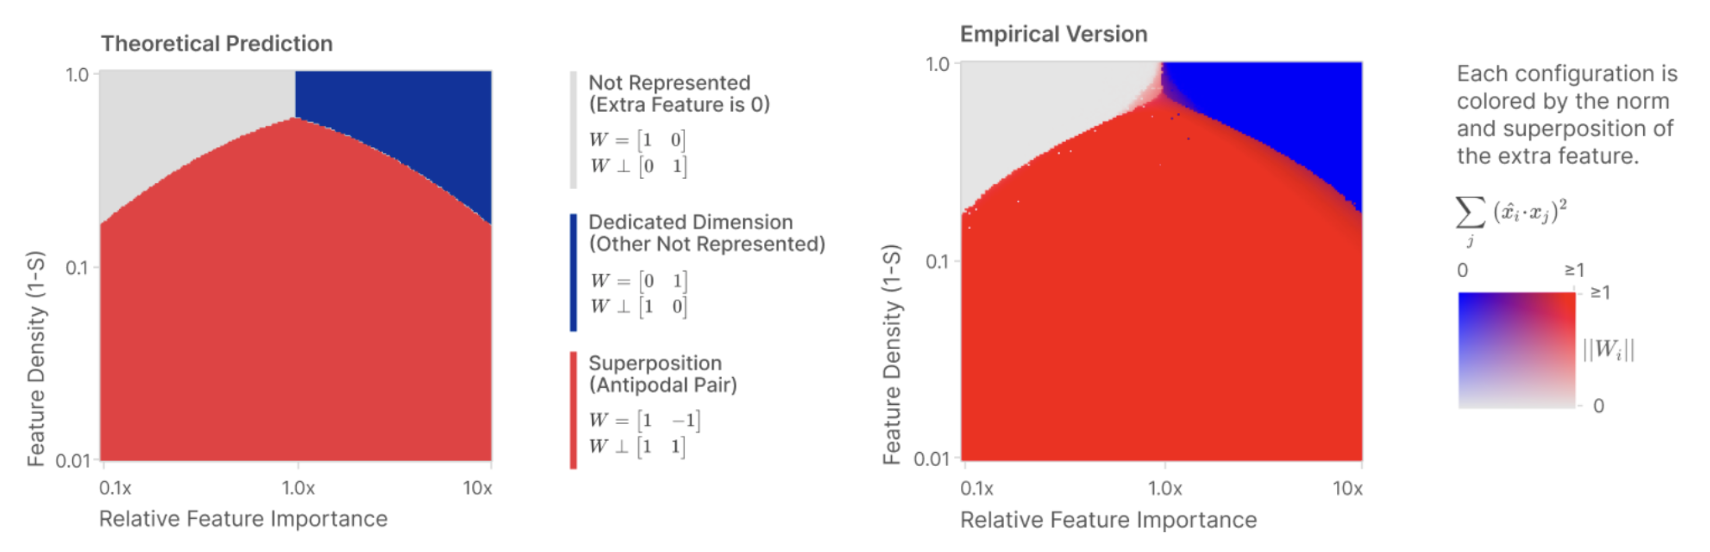
\includegraphics[width=0.99\linewidth]{phase_changes/images/phase_changes_anthropic.png}
    \captionsetup{font=footnotesize, width=0.7\linewidth} % Set the font size for this caption
    \caption{
        Theoretical and empirical superposition in one neuron models in 
        \textit{Toy Models of Superposition}\cite{elhage2022toy}
    }
    \label{fig:section4_anthropic}
\end{figure}

These phase diagrams present three discrete possibilities for the way this single
neuron model represents it's input internally. The colors on the graph represent
which of these internal configurations lead to the lowest theoretical loss.
The first possibility is the model 
\textit{only} represents the first input. In this case, the weight matrix $W = [1, 0]$ (shown in
gray in Figure~\ref{fig:section4_anthropic}). The opposite option is also a 
possibility: the model could only embed the second feature making $W = [0, 1]$ 
(shown in blue). The third possibility is the model could represent \textit{both}
features by making $W = [1, -1]$ (shown in red). \\

The authors claim it is possible to calculate theoretical losses based on sparsity,
relative feature importance, and the weight matrix $W$ for each of these models. 
\textit{Toy Models of Superposition} links to this 
\href{https://github.com/wattenberg/superposition/blob/main/Exploring_Exact_Toy_Models.ipynb}{notebook} 
which specifies the equations for calculating these theoretical losses in 3 
dimensions, but they should work exactly the same in this 2 dimensional example:

\begin{equation}
    \label{eq:loss1}
    \text{Loss for when  $W$ is $[1, 0]$} = \frac{s}{3} - \frac{s^2}{4}
\end{equation}

\begin{equation}
    \label{eq:loss2}
    \text{Loss for when  $W$ is $[0, 1]$} = r \left(\frac{s}{3} - \frac{s^2}{4}\right)
\end{equation}

\begin{equation}
    \label{eq:loss3}
    \text{Loss for when  $W$ is $[1, -1]$} = \frac{(1 + r)s^2}{6}
\end{equation}

The variable $r$ is the relative importance of the second feature. The variable
$s$ is the feature density---in other words, 1 - sparsity. For information
about how these equations were derived, visit the
\href{https://github.com/wattenberg/superposition/blob/main/Exploring_Exact_Toy_Models.ipynb}{notebook} 
provided by the authors.
Based on these equations, the authors were able to plot which weight configuration
would theoretically lead to the lowest loss in Figure~\ref{fig:section4_anthropic}.
They were then able to train models and average the results to show that the
same pattern emerges empirically when training models with gradient descent.

\subsection{Replicating Superposition as a Phase Change}

Replicating the findings from \textit{Toy Models of Superposition} in the
previous subsection was an intricate process that will be described in detail in the
succeeding sections. Figure~\ref{fig:phase_changes_replication} is a visual
summary of my findings. It will be referred to in the subsections below as a
way to clarify my claims.

\begin{figure}[h]
    \centering
    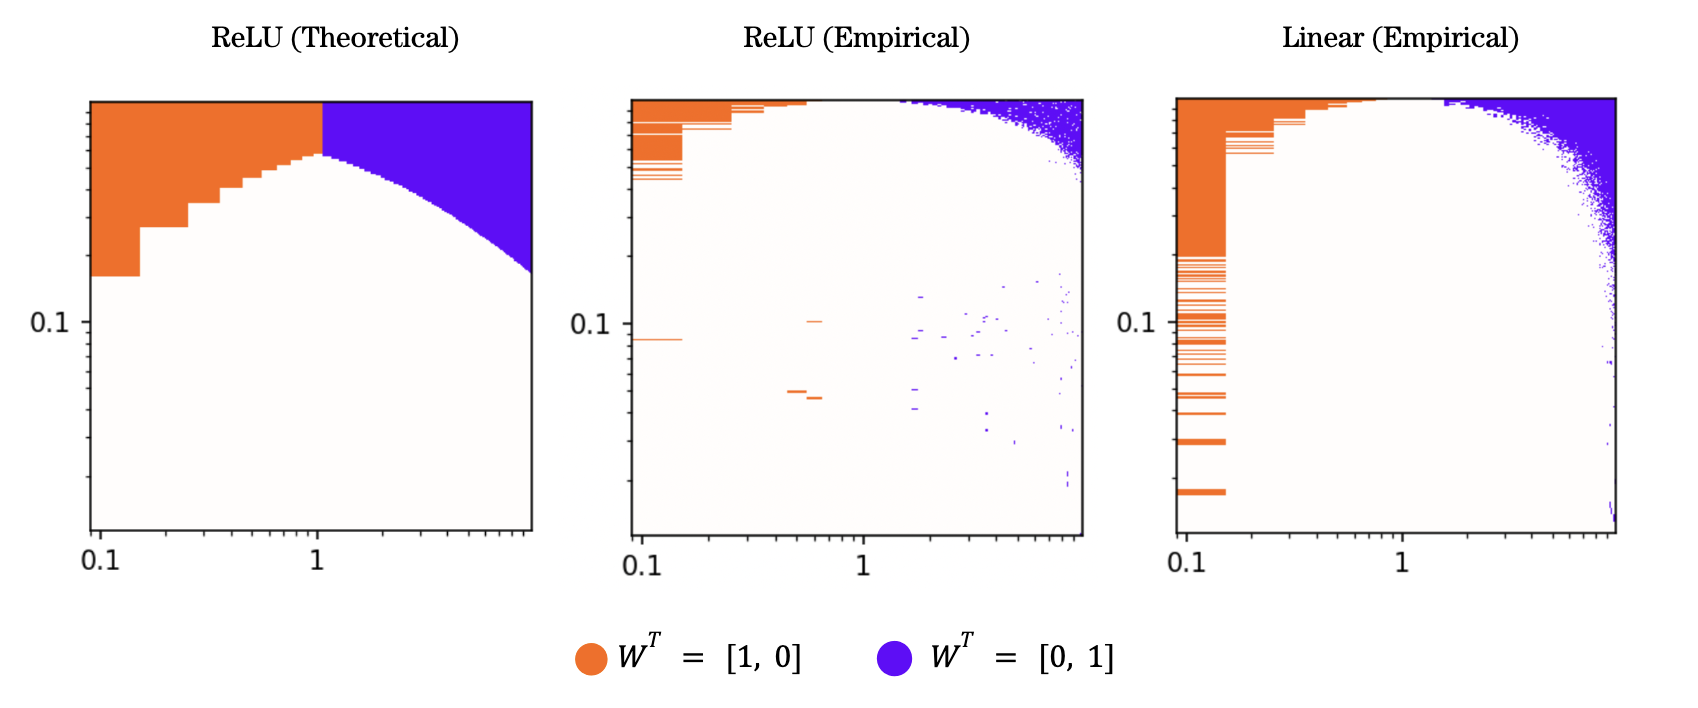
\includegraphics[width=0.99\linewidth]{phase_changes/images/phase_changes_replication.png}
    \captionsetup{font=footnotesize, width=0.7\linewidth} % Set the font size for this caption
    \caption{
        Theoretical and empirical superposition in one-neuron models. Unlike
        the authors of \textit{Toy Models of Superposition}, I perform experiments
        on both models defined by ReLU($W^TWx + b$) and models without an activation
        function. Unlike the original authors however, my results have some extra
        limitations described in section [insert].
    }
    \label{fig:phase_changes_replication}
\end{figure}

Note that the x-axis of the graphs in figure~\ref{fig:phase_changes_replication}
represents the relative ``importance'' of the second output when calculating the
loss. The y-axis represents the ``feature density'' of a model's training data
(that is 1 - sparsity).

\subsection{Replicating Theoretical Predictions}

By using equations~\ref{eq:loss1}, \ref{eq:loss2} and \ref{eq:loss3},
I was able to replicate the theoretical phase diagram from
\textit{Toy Models of Superposition}.
The careful reader however, will notice that the theoretical prediction in
Figure~\ref{fig:section4_anthropic} (graphic from \textit{Toy Models of 
Superposition}) looks far less choppy than the one in Figure~\ref{fig:phase_changes_replication} (graphic
generated for this replication). This is because in the theoretical prediction I 
generated, steps between each value on the x-axis are much larger. This, however, is
intentional and is beneficial for two reasons. First, by creating larger steps 
between numbers on
the x-axis, I was able to intentionally tweak the step size to make the numbers
easiest to work with when generating the graph. It is also beneficial because
larger step sizes means that the graph includes far fewer theoretical
models. This meant that attempting to construct an empirical version of the theoretical graph 
required training fewer real models. Because my current setup is very 
compute-constrained, this made performing the tasks in the following subsections
much more manageable.

\begin{figure}[h]
    \centering
    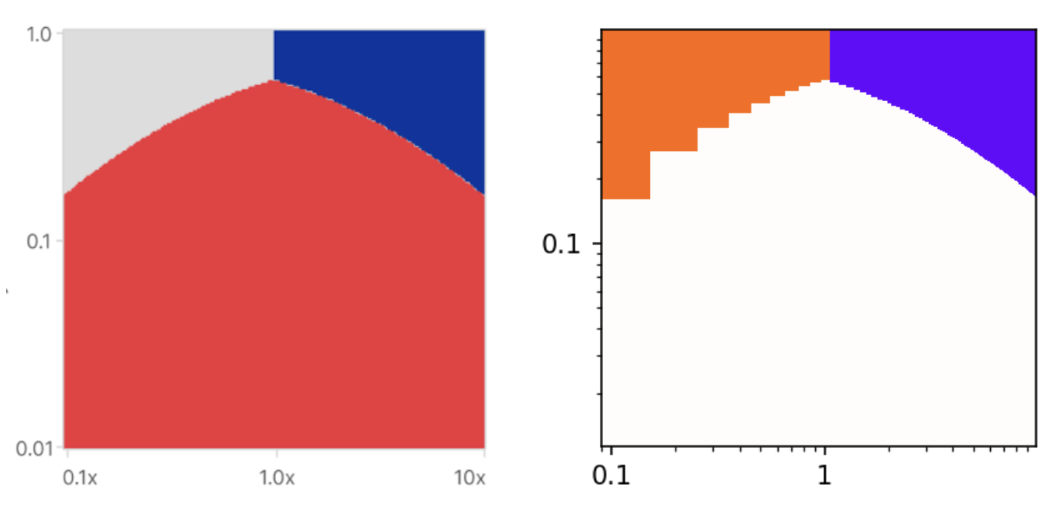
\includegraphics[width=0.5\linewidth]{phase_changes/images/theoretical_predictions.png}
    \captionsetup{font=footnotesize, width=0.7\linewidth} % Set the font size for this caption
    \caption{
        Comparison of theoretical predictions for internal structure of one-neuron 
        models. Figure from \textit{Toy Models of Superposition} is shown on the 
        left while replication for this paper shown on right. 
    }
    \label{fig:theoretical_preditions}
\end{figure}

\textbf{Important Point of Clarification:} Although 
figure~\ref{fig:phase_changes_replication} includes a graph for both linear and ReLU
empirical results, the theoretical predictions are strictly calculated assuming
a ReLU activation function on the model. We discuss the linear findings in section
[insert], but the main focus of this replication is on the ReLU results.

\subsection{Training 1,000,000 ReLU Models}

Theoretical predictions in figure~\ref{fig:phase_changes_replication} account
for 1000 different levels of feature sparsity and 100 levels of relative feature
importance. As a result, in order to test the predictions empirically, it was
necessary to train batches of 100,000 models. In order to create a good sample
to detect trends, I trained 10 batches of 100,000 ReLU models, for a total of one million
models across training. In my compute-constrained environment,
this proved to be a significant challenge. For this reason, I had to make a few
important considerations when writing code to train the ReLU models. I used 
similar methods to train a set of linear models but this is discussed separately
in section [insert].\\

The most obvious thing I did to improve performance when training the 
ReLU models was to not train each model independently. Instead, I constructed a 
PyTorch tensor which included all 100,000 models and used built-in PyTorch functions 
to train the models simultaneously. This helps PyTorch optimize training by 
leveraging features like parallel operations. \\

Another thing I did to make training more efficient was to initialize the weights and
biases in a way that helps each model reduce its loss faster and avoid local minima.
I found it to be highly beneficial to initialize the weights using a normal 
distribution with a standard deviation of 1.5 instead of
1.0 (which perhaps would be a more natural choice in this kind of setup). This change
makes sense because 
in theory, the model should ``want'' to make each item in its weight matrix
either 1 or -1. Increasing the standard deviation puts more numbers around this range.
Similarly, I found that it is advantageous to decrease the standard deviation of the
bias parameters from 1 to 0.5. This makes intuitive sense because
there is no case where the one-neuron models should ``want'' to have large bias values.
It is worth noting that initializing the weights and biases in this way does
not eliminate the need for the models to be trained using gradient descent.
Figure~\ref{fig:relu_loss} shows how even with these weight initializations, the
overall loss of the trained models is still initially very high and quickly
decreases as the models are trained. The goal of initializing the weights and biases
with unconventional standard deviations is not to eliminate the need for training
but to rather help the models achieve lower losses and train more efficiently.

\begin{figure}[h]
    \centering
    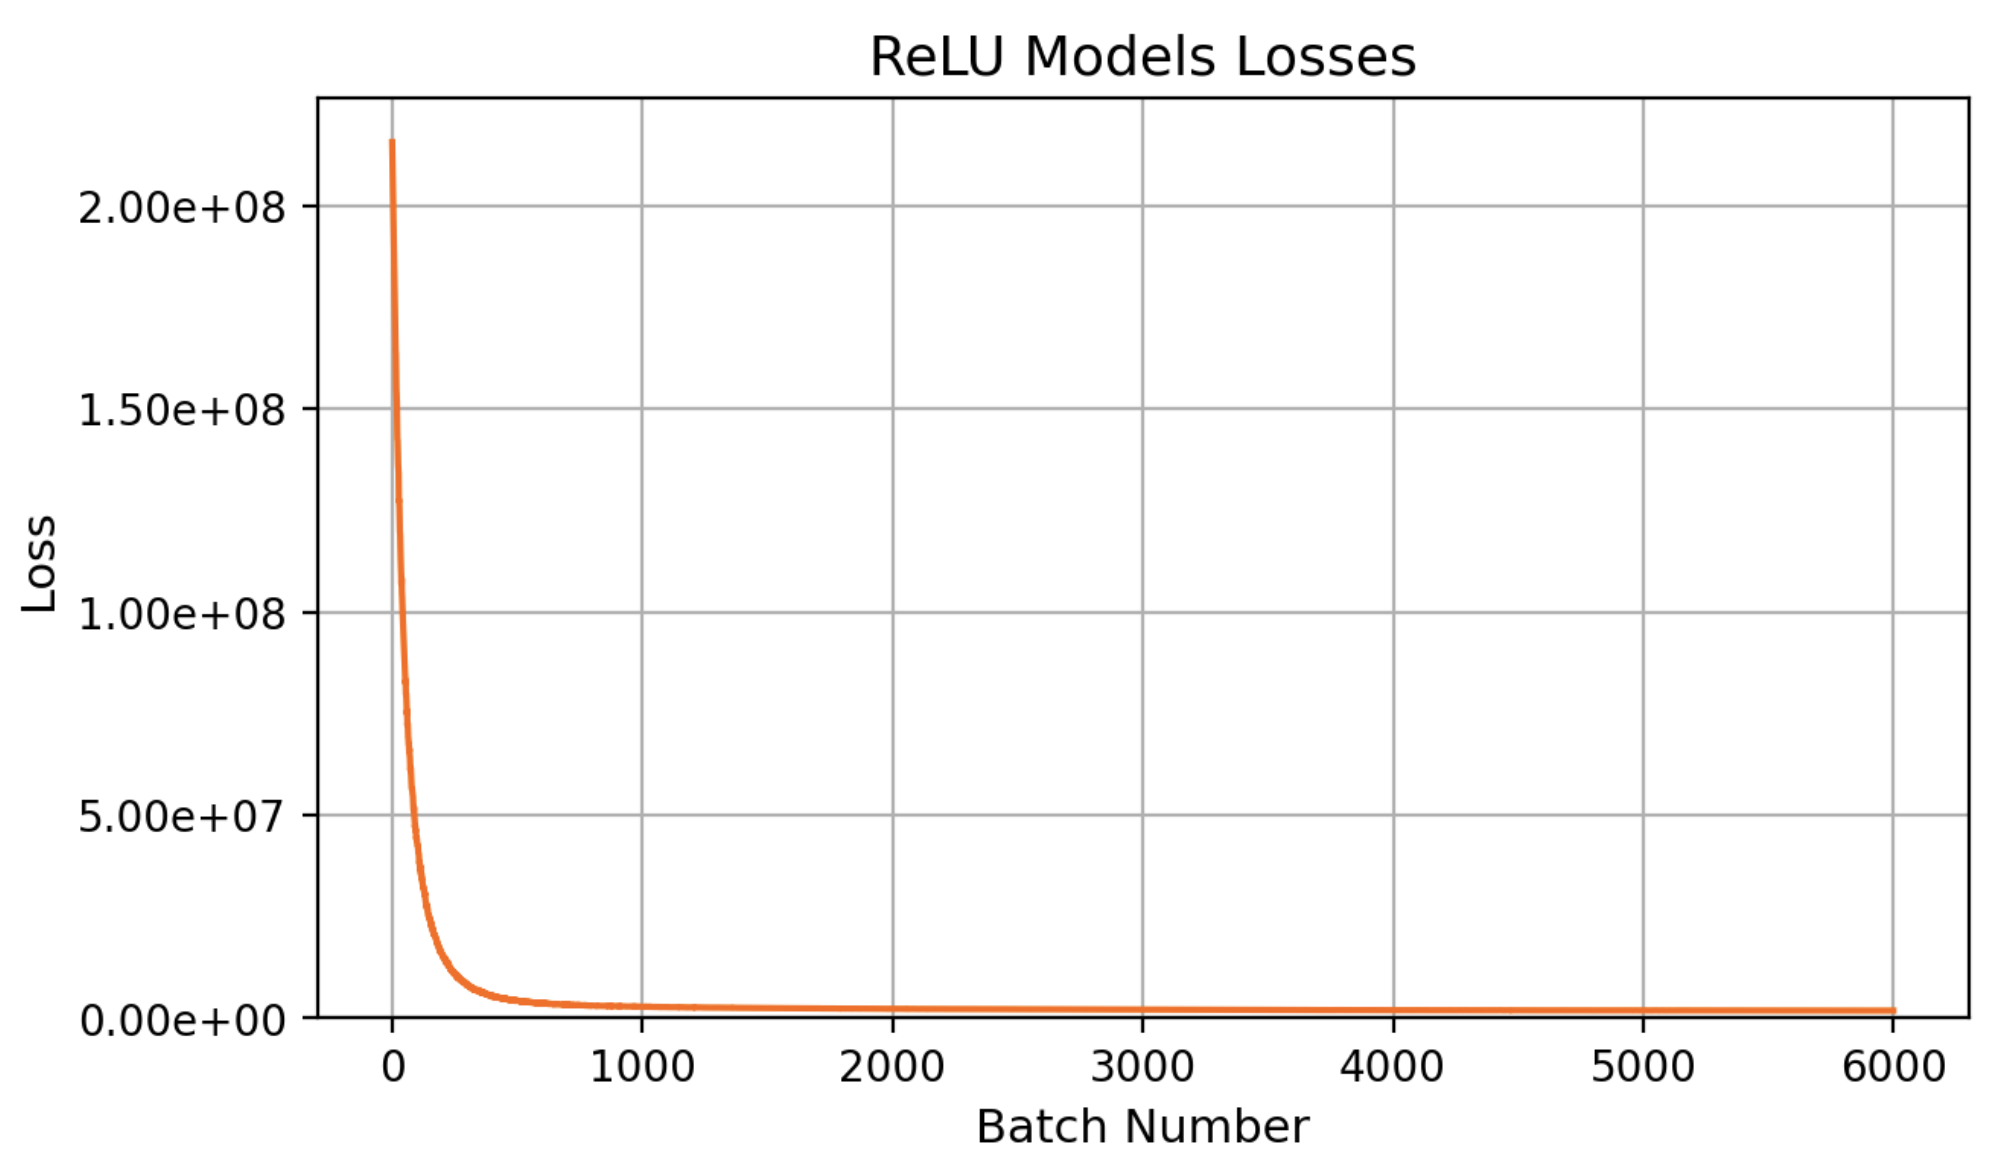
\includegraphics[width=0.5\linewidth]{phase_changes/images/relu_loss.png}
    \captionsetup{font=footnotesize, width=0.7\linewidth} % Set the font size for this caption
    \caption{
        Loss for ReLU models trained in this replication. Note that each point
        on the graph is the loss for a batch of 64 examples of 100,000 models. 
        The x-axis indicates the batch number in training.
    }
    \label{fig:relu_loss}
\end{figure}

The overall result of this training is shown below and compared with the findings
from \textit{Toy Models of Superposition}. Both diagrams show
the empirical result of training one-neuron ReLU toy models.

\begin{figure}[h]
    \centering
    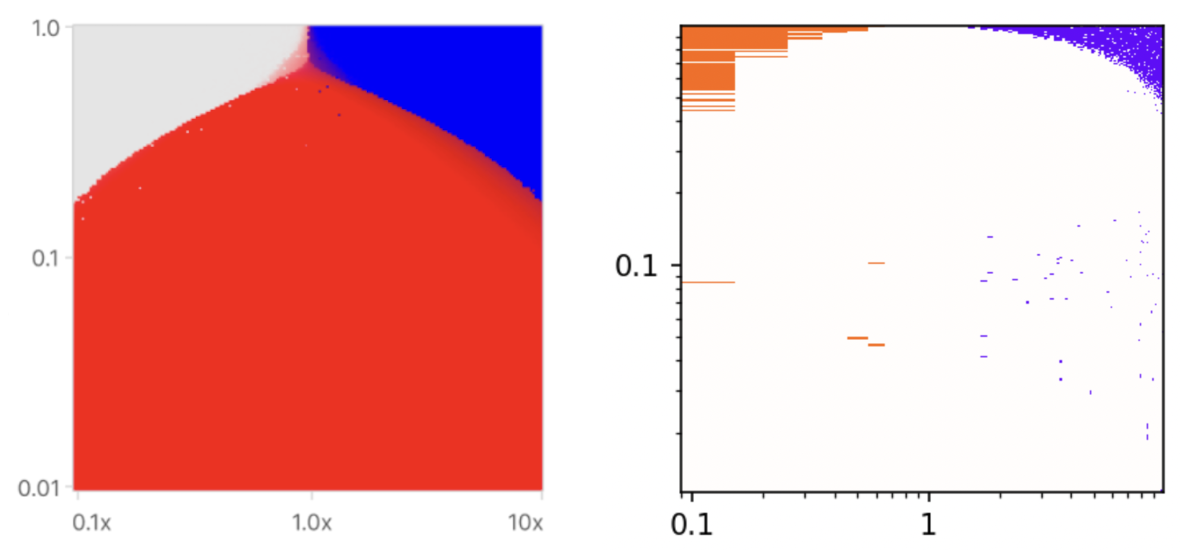
\includegraphics[width=0.5\linewidth]{phase_changes/images/relu_empirical.png}
    \captionsetup{font=footnotesize, width=0.7\linewidth} % Set the font size for this caption
    \caption{
        Empirical losses for one-neuron ReLU toy models. The graph on the left
        is taken from \textit{Toy Models of Superposition}. The figure on the
        right was generated for this replication.
    }
    \label{fig:relu_empirical}
\end{figure}

Although there are a few clear differences between the graphs in
figure~\ref{fig:relu_empirical}, the results are similar in the way that they
each illustrate
analogous overall trends. When a one-neuron ReLU model is trained with high feature
density and with a loss that allocates a very low level of relative
importance to the second output, the model tends to represent
only the first input internally ($W \approx [1, 0]$). If the second feature has 
a high relative importance, only the second input is represented
in $W$ ($W \approx [0, 1]$). As the feature density of the model's training data
decreases, the model has an incentive to not map features in this way but to rather
represent them in superposition. This is the same phenomenon we observed in 
figure~\ref{fig:section1_replication} from the introduction of this paper.\\

There are, however, also clearly a few important differences between the graphs in
figure~\ref{fig:relu_empirical}. The first is that the result generated by the
authors of \textit{Toy Models of Superposition} matches the theoretical
expectation much better than the graph generated for this replication. This could
be partially because of slightly different methods used in interpreting the results
of training these one-neuron models. In the original paper, the authors train
10 batches of real models saying they ``average over the results, discarding 
the model with the highest loss.'' I was not able to follow this exact process
because it is not entirely clear what it means in this context to ``average over
the results.'' Because a model with $W = [1, 0]$ behaves in the exact same way as
a model with
$W = [-1, 0]$ it doesn't make sense to average over the models making 
$W_{avg} = [0, 0]$. Likewise, it does not make sense to take the absolute value
of each weight matrix before averaging because in some cases having a negative
number does make the model behave differently (e.g., $W = [1, -1]$). As a result,
I took a slightly different approach. For each model I trained, I kept track of
whether the weight matrix $W$ represented only the first feature or only the second feature.
If $W$ represented neither or both, I skipped it. At the end of training, if more
than half of the models trained at a given point mapped only the first feature,
that point was colored orange on the resulting graph. If more than half the models
mapped only the second feature,
the point was colored purple. Using this method may have been more strict than
the tactics used by the original authors making my graph more bare and less similar to the
theoretical predictions.\\

Another factor that could have led to a discrepancy between the theoretical
and empirical findings may have been the non-ideal environment in which
one-neuron ReLU models were trained in. Because my setup is compute-constrained,
I was not able to iterate and experiment as much as I wish I could have in training 
the models. As a result, I expect the loss I achieved could have been significantly
lower in an ideal training environment.

\subsection{Training 100,000 Linear Models}

In addition to training a ground of one-neuron ReLU models, I also trained a group
without an activation function. Unlike the group of ReLU models in the previous
section, I only trained each linear model once. This proved to be enough to get
a general idea of how the models behave in practice. \\

In theory these linear models should not exhibit superposition. It is in the best
interest of these linear models to represent only one feature in the weight matrix---
that is $W$ should be $[1,0]$ or $[0, 1]$. In practice, however,
these linear models do not always do exactly what they ``should'' do. Although each model was trained
extensively---6,000 batches of 128 examples---they did not always do what would
limit the loss the most in theory. The outcome looked like 
figure~\ref{fig:linear_phases} where the x-axis is once again relative feature
importance of the second output and the y axis is feature density of the training
data.

\begin{figure}[h]
    \centering
    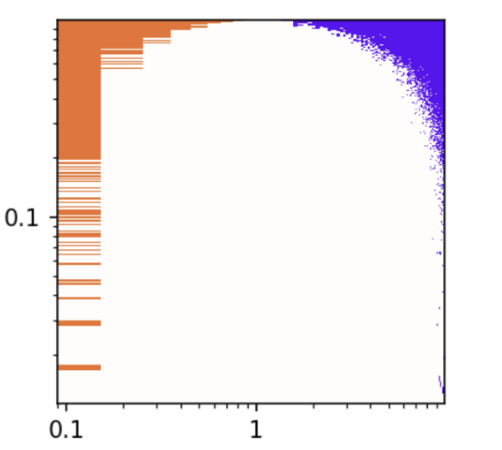
\includegraphics[width=0.25\linewidth]{phase_changes/images/linear_phases.png}
    \captionsetup{font=footnotesize, width=0.7\linewidth} % Set the font size for this caption
    \caption{
        Empirical losses for one-neuron linear toy models.
    }
    \label{fig:linear_phases}
\end{figure}

This example shows something somewhat obvious: even if a model doesn't always do
what is most advantageous for it, it is more likely to do the things it
is incentivized to do. In theory this graph should be all orange and purple. In
practice, however, it only maps features like $[1, 0]$ or $[0, 1]$ when it is
highly favorable. This illustrates a limitation of the research of \textit{Toy 
Models of Superposition}: in practice it can be fairly complex to predict whether
a model should represent a feature in superposition.

\section{Conclusion}

This replication demonstrates that it is possible for models to represent 
features in superposition. It also shows that the phenomenon of superposition is 
somewhat predictable. For example, models trained on sparse data are more
likely to represent the features in superposition. On the other
hand, if one feature is exceedingly important it is very unlikely that that
feature will be represented in superposition. Overall, this replication shows
that there are reasonable frameworks which machine learning researchers can
apply to understand why a model represents information in the way
it does.\\

With that being said, there are some serious limitations to thinking about neural 
networks in this way. In all the examples in this replication, the result was 
highly dependent on the exact training conditions such as learning rate and 
batch size. Thus, I believe that it is wise to be cautious when making broad 
claims about models such as ``model x will represent less information in 
superposition than model y because model x is larger.'' The truth is that there 
are a number of important factors that influence whether or not a model will
represent information orthogonally or in superposition.

\bibliographystyle{plain}
\bibliography{references}

\end{document} % This line marks the end of the document content.
